\documentclass[11pt]{article}

\usepackage[T1]{fontenc}
\usepackage{amsmath}
\usepackage{amssymb}
\usepackage{booktabs}
\usepackage[margin=1in]{geometry}
\usepackage{graphicx}
\usepackage[hidelinks]{hyperref}
\usepackage{microtype}
\usepackage{placeins}
\usepackage{xcolor}
\usepackage{tikz}
\usetikzlibrary{arrows.meta,calc,fit,positioning}

\definecolor{laraBlue}{HTML}{2D6A9F}
\definecolor{laraBlueLight}{HTML}{E8F2F8}
\definecolor{laraGreen}{HTML}{3E8060}
\definecolor{laraGreenLight}{HTML}{EAF5EF}
\definecolor{laraOrange}{HTML}{B76B24}
\definecolor{laraOrangeLight}{HTML}{FBF0E4}
\definecolor{laraPurple}{HTML}{74549B}
\definecolor{laraPurpleLight}{HTML}{F0EBF7}
\definecolor{laraGray}{HTML}{4F5B66}

\tikzset{
  flow/.style={-{Stealth[length=2mm]}, semithick, draw=laraGray},
  petri arc/.style={-{Stealth[length=1.8mm]}, thick, draw=laraGray},
  data box/.style={draw=laraBlue, fill=laraBlueLight, rounded corners=2pt,
    align=center, minimum height=7mm, inner xsep=5pt, inner ysep=3pt},
  process box/.style={draw=laraGreen, fill=laraGreenLight,
    rounded corners=2pt, align=center, minimum height=7mm,
    inner xsep=5pt, inner ysep=3pt},
  decision box/.style={draw=laraOrange, fill=laraOrangeLight,
    rounded corners=2pt, align=center, minimum height=7mm,
    inner xsep=5pt, inner ysep=3pt},
  output box/.style={draw=laraPurple, fill=laraPurpleLight,
    rounded corners=2pt, align=center, minimum height=7mm,
    inner xsep=5pt, inner ysep=3pt},
  panel/.style={draw=black!25, rounded corners=3pt, fill=black!1,
    inner sep=6pt},
  place/.style={circle, draw=laraGray, thick, fill=white,
    minimum size=5.5mm, inner sep=0pt},
  marked place/.style={place, font=\scriptsize},
  visible transition/.style={rectangle, draw=laraBlue, thick,
    fill=laraBlueLight, minimum width=6mm, minimum height=6mm,
    inner sep=1pt, font=\scriptsize\sffamily},
  silent transition/.style={rectangle, draw=laraGray, thick,
    fill=laraGray, text=white, minimum width=3.5mm,
    minimum height=6mm, inner sep=0pt, font=\scriptsize\sffamily},
  event/.style={draw=laraBlue, fill=laraBlueLight, rounded corners=1.5pt,
    minimum width=7mm, minimum height=6mm, inner sep=1pt,
    font=\scriptsize\sffamily},
  operation/.style={draw=laraOrange, fill=laraOrangeLight,
    rounded corners=1.5pt, align=center, minimum height=6mm,
    inner xsep=4pt, font=\scriptsize\sffamily},
  tiny label/.style={font=\scriptsize\sffamily, text=laraGray}
}

\setlength{\emergencystretch}{2em}

\title{LARA: Training Inputs, Data Generation, and Losses}
\author{Alessandro Berti \and Wil M. P. van der Aalst}
\date{}

\begin{document}

\maketitle

\appendix

\section{Training Data Generation}
\label{app:data-generation}

This standalone appendix specifies the concrete network inputs and training
targets, expands the data generation procedure, and gives the complete loss
used by the reference run. The data generator creates a
supervised alignment corpus in which every row contains a Petri net, one trace,
and the exact optimal alignment for that trace on that net. The relevant code
path is \texttt{scripts/init\_data.py}, which calls the behavior-family
generator in \texttt{lara\_align/families.py}, the PM4Py exact aligner in
\texttt{lara\_align/exact.py}, and the replay verifier in
\texttt{lara\_align/verify.py}. The checked-in reference corpus uses dataset
format version 2 and the defaults represented in
\texttt{configs/behavior\_families.json}.

\subsection{What One Training Row Contains}

One generated row is an \texttt{AlignmentSample}. It contains:
\begin{itemize}
  \item a unique sample id and its split;
  \item a Petri net $SN$ with its initial and final markings;
  \item one observed trace $\sigma$;
  \item an optimal alignment $\gamma^\ast$ computed by the exact backend;
  \item the optimal cost $\delta = c(\gamma^\ast)$ under the standard move
    costs;
  \item metadata describing how the row was generated.
\end{itemize}
The standard costs are the same costs used throughout the paper: synchronous
moves cost zero, visible log moves cost one, visible model moves cost one, and
silent model moves cost zero. The exact alignment is transition-aware. Thus a
synchronous move stores the concrete transition name, not only the visible
activity label. This matters when two transitions have the same label.

The network receives only numeric features of the net, its markings and labels,
and the observed trace. Sample IDs, family metadata, the clean trace, the exact
alignment, and its cost are not input features. The neural training targets are
derived from this exact alignment. For each
trace event, the sync target is the transition fired by the exact alignment
when that event is synchronized. Events skipped by the optimum become log-move
targets. Transitions fired without consuming an event become model-move
targets. The exact cost is also stored as the target for the learned cost
estimate.

\subsection{A Concrete Stored Training Input}
\label{app:concrete-input}

Consider \texttt{train-000048} in \texttt{data/lara\_synthetic/train.pkl}
(seed 13, dataset version 2). It belongs to the duplicate-prefix representation
of family \texttt{train-6fda2acef53502aa}. The generator selected the clean trace
$\langle A,B,D,E\rangle$, swapped the last two events, and substituted $C$ for
$B$, yielding the observed input $\sigma=\langle A,C,E,D\rangle$. The two
representations of this family both admit exactly $ABDE$ and $ACDE$; the same
observation is separately aligned on each representation.

For readability, write $A_L,A_R,B,C,D,E$ for transition identities, with
$\lambda(A_L)=\lambda(A_R)=A$ and the other labels equal to the displayed
letters. The complete input net has six places and six transitions. Its paths
are
\[
 p_0\xrightarrow{A_L}p_L\xrightarrow{B}p_f
 \xrightarrow{D}p_D\xrightarrow{E}p_E,
 \qquad p_0\xrightarrow{A_R}p_R\xrightarrow{C}p_f.
\]
All arcs have weight one. The initial marking is $[p_0]$ and the final marking
is $[p_E]$; $p_f$ is only the end of the core, before the shared suffix.
Table~\ref{tab:stored-order} fixes the actual sorted tensor order and connects
the readable notation to the stored identifiers. Names fix indices but are not
embedded as semantic features.

\begin{table}[htbp]
\centering
\small
\caption{Stored identifier order for \texttt{train-000048}. Node indices put
places first; transition target indices are zero-based within the transition list.}
\label{tab:stored-order}
\setlength{\tabcolsep}{3pt}
\begin{tabular}{@{}rll|rll@{}}
\toprule
node & place & stored name & target index & transition & stored name\\
\midrule
0 & $p_D$ & \texttt{context\_sink\_000} & 0 & $D$ & \texttt{context\_000\_D}\\
1 & $p_E$ & \texttt{context\_sink\_001} & 1 & $E$ & \texttt{context\_001\_E}\\
2 & $p_0$ & \texttt{p0} & 2 & $A_L$ & \texttt{t\_A\_left}\\
3 & $p_f$ & \texttt{pf} & 3 & $A_R$ & \texttt{t\_A\_right}\\
4 & $p_L$ & \texttt{pl} & 4 & $B$ & \texttt{t\_B}\\
5 & $p_R$ & \texttt{pr} & 5 & $C$ & \texttt{t\_C}\\
\bottomrule
\end{tabular}
\end{table}

\paragraph{Input tensors.}
\texttt{pm4py\_to\_features} in \texttt{lara\_align/features.py} produces the
input tuple $X=(X_P,X_T,E,r,z_T,z_\sigma,C)$. A place row is
$(m_0,m_f,d^-,d^+,d^-+d^+)$; a transition row is
$(\mathbf{1}_{\tau},d^-,d^+,c_M,c_S,s)$, where $s$ records a shared input/output
place. For this row,
\[
 X_P=\begin{bmatrix}
 0&0&1&1&2\\0&1&1&0&1\\1&0&0&2&2\\
 0&0&2&1&3\\0&0&1&1&2\\0&0&1&1&2
 \end{bmatrix},\qquad
 X_T=\begin{bmatrix}
 0&1&1&1&0&0\\0&1&1&1&0&0\\0&1&1&1&0&0\\
 0&1&1&1&0&0\\0&1&1&1&0&0\\0&1&1&1&0&0
 \end{bmatrix}.
\]
The transition graph nodes are $6,\ldots,11$ in target-index order. The
following table determines every column of $E$ and every edge type $r$.
For each row $(p,t,q)$, append the four directed edges
$(p,t),(t,p),(t,q),(q,t)$, with types $(0,2,1,3)$ respectively. Types $0,1$
follow consumption and production arcs; types $2,3$ reverse them. Thus $E$ is $2\times24$; $r$ repeats $(0,2,1,3)$ six times.
\[
\begin{array}{c|rrr}
\text{transition}&p&t&q\\\hline
D&3&6&0\\ E&0&7&1\\ A_L&2&8&4\\ A_R&2&9&5\\
B&4&10&3\\ C&5&11&3
\end{array}
\]
For visible labels, the hash is
$h(a)=1+(\operatorname{int}(\operatorname{BLAKE2b}_8(\operatorname{UTF8}(a)))
\bmod8191)$, using an unsigned big-endian integer; $h(\tau)=0$. The integer
input vectors before augmentation are
\[
 z_T=(2587,4475,8075,8075,6408,5878),\qquad
 z_\sigma=(8075,5878,4475,2587).
\]
The shared embedding matrix has 8{,}192 learned rows, each of dimension 96.
An ID selects one row; it is neither an activity count nor a numeric measure
of similarity. Event positions $(0,1,2,3)$ index a separate learned position
embedding. Exact equality of the original visible labels gives
\[
 C=\begin{bmatrix}
 0&0&1&1&0&0\\0&0&0&0&0&1\\0&1&0&0&0&0\\1&0&0&0&0&0
 \end{bmatrix}.
\]
For example, the first event matches both $A$ transitions; the third event
matches $E$ even though $E$ is not enabled at the initial marking. Compatibility
is a label relation, not an enabledness relation. All seven input tensors are
now specified; no alignment or intermediate marking is supplied to the scorer.

\paragraph{Exact witness and target tensors.}
The stored optimal witness is
\[
 \gamma^*=\langle(A,A_R),(C,C),(E,\gg),(D,D),(\gg,E)\rangle,
 \qquad\delta=2.
\]
It skips the observed $E$, synchronizes the final observed $D$, and completes
with a model move $E$. Both the log move and visible model move cost one.
An alternative optimum inserts model move $D$ before synchronizing the observed
$E$ and skips the last observed $D$. Training uses the stored witness, not all
optimal witnesses simultaneously.

With the transition indices in Table~\ref{tab:stored-order},
\texttt{targets\_from\_alignment} in \texttt{lara\_align/training.py} returns
\[
 y=(3,5,-1,0),\qquad q=(0,0,1,0),\qquad
 b=(0,1,0,0,0,0),\qquad\delta=2.
\]
Here $y$ is an integer tensor of length four, $q$ a binary event target of
length four, $b$ a binary transition target of length six, and $\delta$ a scalar.
The value $-1$ excludes that event from synchronous cross-entropy. A positive
$b_j$ means that transition $j$ occurs at least once as a model move, including
silent moves when present; it gives neither the position nor the number of
such occurrences. These are supervision tensors, separate from $X$.
The row contains $C$ but not $B$, so transition-identity supervision is active.

\paragraph{Training-time relabeling.}
Each training visit independently remaps label IDs with probability $0.5$.
The implementation draws distinct replacement IDs from $1,\ldots,8191$ for
the distinct nonzero IDs appearing in the net and trace, and applies the same
mapping to both vectors. For example, the assignment
$8075\mapsto101$, $6408\mapsto205$, $5878\mapsto309$,
$2587\mapsto413$, $4475\mapsto517$ would give
$z_T'=(413,517,101,101,205,309)$ and
$z_\sigma'=(101,309,517,413)$. This is an illustrative augmentation, not the
recorded random draw. The graph, $C$, and all targets are unchanged; ID zero
remains reserved for silent transitions. Existing hash collisions remain
collisions. This trains reuse across activity vocabularies without claiming
exact invariance to every label renaming. Validation and test use unmodified
hash IDs.

\FloatBarrier

\subsection{Behavior Families}

The generator does not create isolated trace and net pairs directly. It first
creates a \emph{behavior family}. Formally, a family fixes two labeled system nets $SN_1,SN_2$ whose
complete visible languages agree, $L(SN_1)=L(SN_2)=L$, and two observations
$\sigma_1,\sigma_2$ obtained by corrupting traces from $L$. An observation
need not itself belong to $L$. This is the unit that is assigned to train, validation, or test
before any row is written. Assigning whole families to a split keeps the four rows of a generated
family together. It does not make motif classes or all visible languages
disjoint across splits: independently generated families can share a language.

With the default configuration, each family has two Petri net representations
and two observed traces. Therefore each family expands to four rows:
\[
  2 \text{ representations} \times 2 \text{ traces} = 4 \text{ rows}.
\]

\begin{figure}[htbp]
\centering
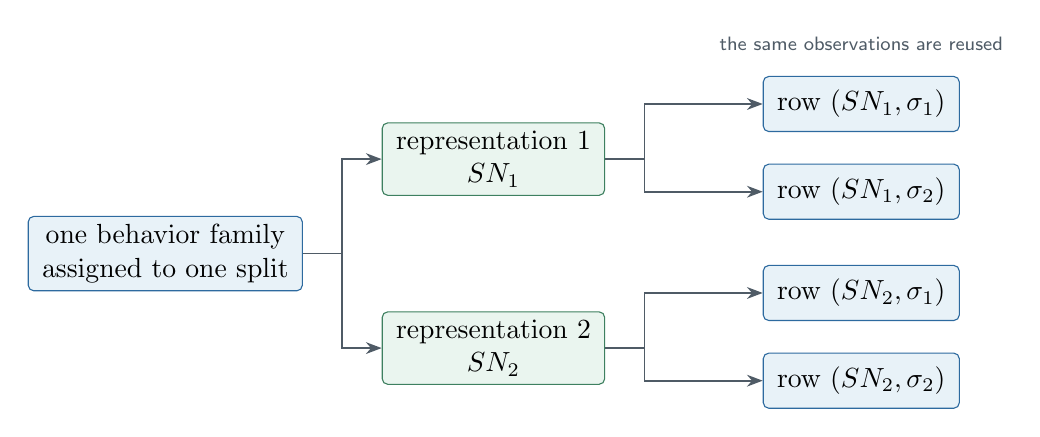
\begin{tikzpicture}[node distance=7mm and 10mm]
  \node[data box, minimum width=31mm] (family)
    {one behavior family\\assigned to one split};
  \node[process box, right=of family, yshift=12mm] (r1)
    {representation 1\\$SN_1$};
  \node[process box, right=of family, yshift=-12mm] (r2)
    {representation 2\\$SN_2$};
  \node[data box, right=20mm of r1, yshift=7mm] (r1t1)
    {row $(SN_1,\sigma_1)$};
  \node[data box, below=4mm of r1t1] (r1t2)
    {row $(SN_1,\sigma_2)$};
  \node[data box, right=20mm of r2, yshift=7mm] (r2t1)
    {row $(SN_2,\sigma_1)$};
  \node[data box, below=4mm of r2t1] (r2t2)
    {row $(SN_2,\sigma_2)$};
  \draw[flow] (family.east) -- ++(5mm,0) |- (r1.west);
  \draw[flow] (family.east) -- ++(5mm,0) |- (r2.west);
  \draw[flow] (r1.east) -- ++(5mm,0) |- (r1t1.west);
  \draw[flow] (r1.east) -- ++(5mm,0) |- (r1t2.west);
  \draw[flow] (r2.east) -- ++(5mm,0) |- (r2t1.west);
  \draw[flow] (r2.east) -- ++(5mm,0) |- (r2t2.west);
  \node[tiny label, above=2mm of r1t1] {the same observations are reused};
\end{tikzpicture}
\caption{Expansion of one behavior family into four supervised rows. The split
is chosen at family level, and both representations receive the same two
observed traces.}
\label{fig:family-expansion}
\end{figure}

The reference corpus uses four family motifs with equal weight. Table
\ref{tab:appendix-motifs} summarizes them.

Before generation, the requested family count is converted into a deterministic
motif quota. The quota reserves the configured per-motif minimum, distributes
the remaining families according to the motif weights, and shuffles the plan
with a split-specific seed. If an attempted family is rejected, the next family
index is tried for the same planned motif. Consequently, rejection does not
silently change the requested class balance. The family id, rather than an
individual row id, is the split key.

\begin{table}
\centering
\caption{Behavior-family motifs used in the reference corpus. Each family
contains two Petri net representations of the same visible behavior.}
\label{tab:appendix-motifs}
\small
\begin{tabular}{@{}lll@{}}
\toprule
motif & representation 1 & representation 2 \\
\midrule
ordinary tree & canonical block net & isomorphic renaming \\
duplicate versus silent & duplicate-prefix net & silent-routing net \\
concurrent versus interleaved & parallel net & explicit interleaving net \\
M-pattern & canonical block net & non-free-choice M-pattern net \\
\bottomrule
\end{tabular}
\end{table}

\paragraph{Ordinary Tree.}
The ordinary-tree motif samples a random block-structured process tree. The
default tree has between 4 and 12 visible activity occurrences and depth at
most 6. Internal nodes are sampled from sequence, exclusive choice, and
parallel composition with weights 0.4, 0.3, and 0.3. The visible alphabet size
is about 70\% of the number of visible occurrences, so duplicate labels can
appear naturally. The first representation is the compiled block-structured
Petri net. The second representation is an isomorphic renaming of the same net:
places and transition names are changed, but labels and behavior are preserved.

Figure \ref{fig:ordinary-tree-pair} uses a small sampled tree to illustrate the
transformation. In the Petri net figures, circles are places, blue rectangles
are visible transitions, dark rectangles are silent transitions, and a bullet
marks the initial token.

\begin{figure}[htbp]
\centering
\resizebox{\textwidth}{!}{%
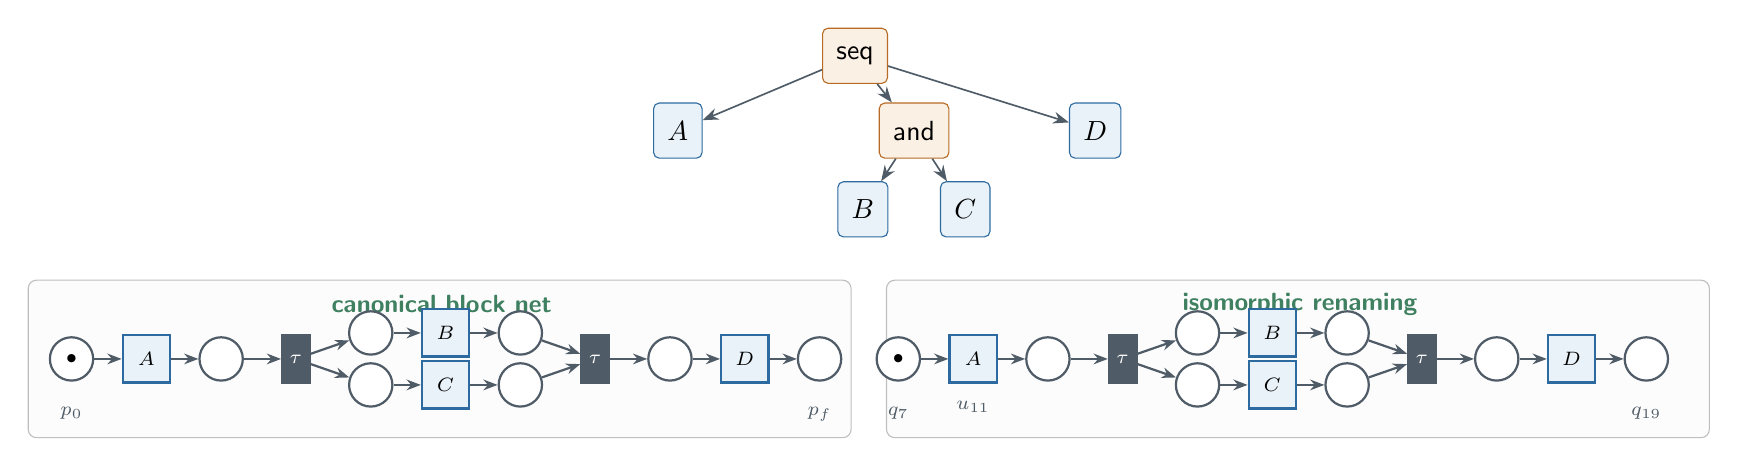
\begin{tikzpicture}
  \node[decision box] (seq) at (10.05,2.8) {$\mathsf{seq}$};
  \node[data box] (ta) at (7.8,1.85) {$A$};
  \node[decision box] (and) at (10.8,1.85) {$\mathsf{and}$};
  \node[data box] (td) at (13.1,1.85) {$D$};
  \node[data box] (tb) at (10.15,0.85) {$B$};
  \node[data box] (tc) at (11.45,0.85) {$C$};
  \draw[flow] (seq) -- (ta);
  \draw[flow] (seq) -- (and);
  \draw[flow] (seq) -- (td);
  \draw[flow] (and) -- (tb);
  \draw[flow] (and) -- (tc);

  \draw[draw=black!25, rounded corners=3pt, fill=black!1]
    (-0.45,-2.05) rectangle (10.0,-0.05);
  \node[font=\small\sffamily\bfseries, text=laraGreen] at (4.8,-0.35)
    {canonical block net};
  \node[marked place] (l0) at (0.1,-1.05) {$\bullet$};
  \node[visible transition] (la) at (1.05,-1.05) {$A$};
  \node[place] (l1) at (2.0,-1.05) {};
  \node[silent transition] (ls) at (2.95,-1.05) {$\tau$};
  \node[place] (lpb) at (3.9,-0.72) {};
  \node[place] (lpc) at (3.9,-1.38) {};
  \node[visible transition] (lb) at (4.85,-0.72) {$B$};
  \node[visible transition] (lc) at (4.85,-1.38) {$C$};
  \node[place] (lqb) at (5.8,-0.72) {};
  \node[place] (lqc) at (5.8,-1.38) {};
  \node[silent transition] (lj) at (6.75,-1.05) {$\tau$};
  \node[place] (lf) at (7.7,-1.05) {};
  \node[visible transition] (ld) at (8.65,-1.05) {$D$};
  \node[place] (lff) at (9.6,-1.05) {};
  \draw[petri arc] (l0) -- (la); \draw[petri arc] (la) -- (l1);
  \draw[petri arc] (l1) -- (ls);
  \draw[petri arc] (ls) -- (lpb); \draw[petri arc] (ls) -- (lpc);
  \draw[petri arc] (lpb) -- (lb); \draw[petri arc] (lb) -- (lqb);
  \draw[petri arc] (lpc) -- (lc); \draw[petri arc] (lc) -- (lqc);
  \draw[petri arc] (lqb) -- (lj); \draw[petri arc] (lqc) -- (lj);
  \draw[petri arc] (lj) -- (lf);
  \draw[petri arc] (lf) -- (ld); \draw[petri arc] (ld) -- (lff);
  \node[tiny label, below=2mm of l0] {$p_0$};
  \node[tiny label, below=2mm of lff] {$p_f$};

  \draw[draw=black!25, rounded corners=3pt, fill=black!1]
    (10.45,-2.05) rectangle (20.9,-0.05);
  \node[font=\small\sffamily\bfseries, text=laraGreen] at (15.7,-0.35)
    {isomorphic renaming};
  \node[marked place] (r0) at (10.6,-1.05) {$\bullet$};
  \node[visible transition] (ra) at (11.55,-1.05) {$A$};
  \node[place] (r1) at (12.5,-1.05) {};
  \node[silent transition] (rs) at (13.45,-1.05) {$\tau$};
  \node[place] (rpb) at (14.4,-0.72) {};
  \node[place] (rpc) at (14.4,-1.38) {};
  \node[visible transition] (rb) at (15.35,-0.72) {$B$};
  \node[visible transition] (rc) at (15.35,-1.38) {$C$};
  \node[place] (rqb) at (16.3,-0.72) {};
  \node[place] (rqc) at (16.3,-1.38) {};
  \node[silent transition] (rj) at (17.25,-1.05) {$\tau$};
  \node[place] (rf) at (18.2,-1.05) {};
  \node[visible transition] (rd) at (19.15,-1.05) {$D$};
  \node[place] (rff) at (20.1,-1.05) {};
  \draw[petri arc] (r0) -- (ra); \draw[petri arc] (ra) -- (r1);
  \draw[petri arc] (r1) -- (rs);
  \draw[petri arc] (rs) -- (rpb); \draw[petri arc] (rs) -- (rpc);
  \draw[petri arc] (rpb) -- (rb); \draw[petri arc] (rb) -- (rqb);
  \draw[petri arc] (rpc) -- (rc); \draw[petri arc] (rc) -- (rqc);
  \draw[petri arc] (rqb) -- (rj); \draw[petri arc] (rqc) -- (rj);
  \draw[petri arc] (rj) -- (rf);
  \draw[petri arc] (rf) -- (rd); \draw[petri arc] (rd) -- (rff);
  \node[tiny label, below=2mm of r0] {$q_7$};
  \node[tiny label, below=2mm of rff] {$q_{19}$};
  \node[tiny label, below=1mm of ra] {$u_{11}$};
\end{tikzpicture}%
}
\caption{Illustrative ordinary-tree family for
$\mathsf{seq}(A,\mathsf{and}(B,C),D)$. The second net preserves all arcs and
visible labels while changing place and transition identities. Both nets have
the complete visible language
$\{\langle A,B,C,D\rangle,\langle A,C,B,D\rangle\}$.}
\label{fig:ordinary-tree-pair}
\end{figure}

\paragraph{Duplicate Versus Silent.}
This motif has two ways to represent the visible behavior ``$A$ followed by
either $B$ or $C$''. In the duplicate-prefix representation, there are two
different visible transitions labeled $A$: one leads to the $B$ branch and the
other to the $C$ branch. In the silent-routing representation, there is one
visible $A$ transition followed by a silent choice between the two branches.
This motif directly tests whether the model learns transition identity rather
than only label identity.

\begin{figure}[htbp]
\centering
\resizebox{\textwidth}{!}{%
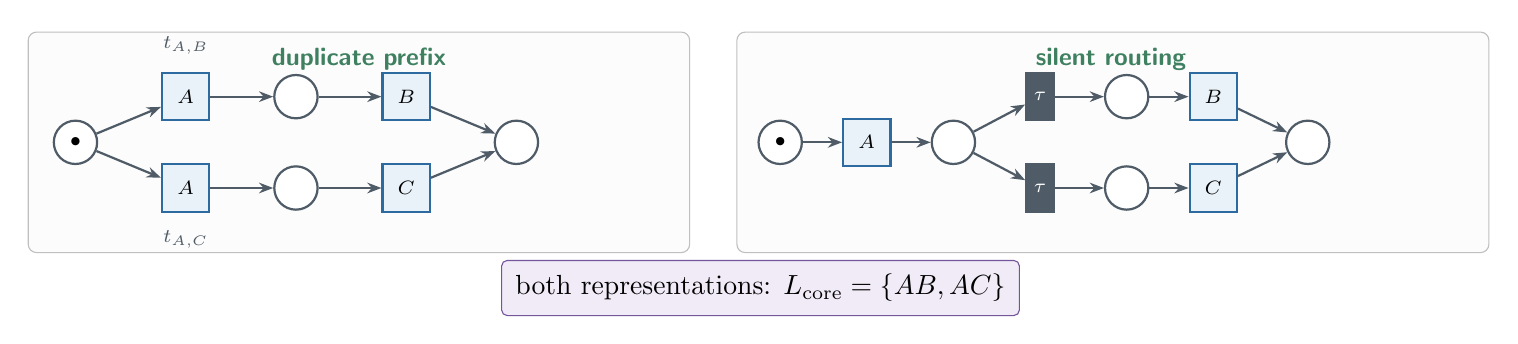
\begin{tikzpicture}
  \draw[draw=black!25, rounded corners=3pt, fill=black!1]
    (-0.45,-1.4) rectangle (7.95,1.4);
  \node[font=\small\sffamily\bfseries, text=laraGreen] at (3.75,1.05)
    {duplicate prefix};
  \node[marked place] (d0) at (0.15,0) {$\bullet$};
  \node[visible transition] (dab) at (1.55,0.58) {$A$};
  \node[visible transition] (dac) at (1.55,-0.58) {$A$};
  \node[place] (dpb) at (2.95,0.58) {};
  \node[place] (dpc) at (2.95,-0.58) {};
  \node[visible transition] (db) at (4.35,0.58) {$B$};
  \node[visible transition] (dc) at (4.35,-0.58) {$C$};
  \node[place] (df) at (5.75,0) {};
  \draw[petri arc] (d0) -- (dab); \draw[petri arc] (d0) -- (dac);
  \draw[petri arc] (dab) -- (dpb); \draw[petri arc] (dac) -- (dpc);
  \draw[petri arc] (dpb) -- (db); \draw[petri arc] (dpc) -- (dc);
  \draw[petri arc] (db) -- (df); \draw[petri arc] (dc) -- (df);
  \node[tiny label, above=1mm of dab] {$t_{A,B}$};
  \node[tiny label, below=1mm of dac] {$t_{A,C}$};

  \draw[draw=black!25, rounded corners=3pt, fill=black!1]
    (8.55,-1.4) rectangle (18.1,1.4);
  \node[font=\small\sffamily\bfseries, text=laraGreen] at (13.3,1.05)
    {silent routing};
  \node[marked place] (s0) at (9.1,0) {$\bullet$};
  \node[visible transition] (sa) at (10.2,0) {$A$};
  \node[place] (s1) at (11.3,0) {};
  \node[silent transition] (stb) at (12.4,0.58) {$\tau$};
  \node[silent transition] (stc) at (12.4,-0.58) {$\tau$};
  \node[place] (spb) at (13.5,0.58) {};
  \node[place] (spc) at (13.5,-0.58) {};
  \node[visible transition] (sb) at (14.6,0.58) {$B$};
  \node[visible transition] (sc) at (14.6,-0.58) {$C$};
  \node[place] (sf) at (15.8,0) {};
  \draw[petri arc] (s0) -- (sa); \draw[petri arc] (sa) -- (s1);
  \draw[petri arc] (s1) -- (stb); \draw[petri arc] (s1) -- (stc);
  \draw[petri arc] (stb) -- (spb); \draw[petri arc] (stc) -- (spc);
  \draw[petri arc] (spb) -- (sb); \draw[petri arc] (spc) -- (sc);
  \draw[petri arc] (sb) -- (sf); \draw[petri arc] (sc) -- (sf);
  \node[output box] at (8.85,-1.85)
    {both representations: $L_{\mathrm{core}}=\{AB,AC\}$};
\end{tikzpicture}%
}
\caption{Two representations of the duplicate-versus-silent motif. The left
net contains two concrete transitions with label $A$; the right net contains
one $A$ transition and a silent choice.}
\label{fig:duplicate-silent-pair}
\end{figure}

\paragraph{Concurrent Versus Interleaved.}
This motif represents the visible language $\langle A,B\rangle$ and
$\langle B,A\rangle$ in two different ways. One representation uses real
parallelism: an invisible split produces two concurrent branches, and an
invisible join closes them. The other representation encodes the two possible
orders explicitly as alternatives. The two nets have the same visible complete
traces but different causal structure.

\begin{figure}[htbp]
\centering
\resizebox{\textwidth}{!}{%
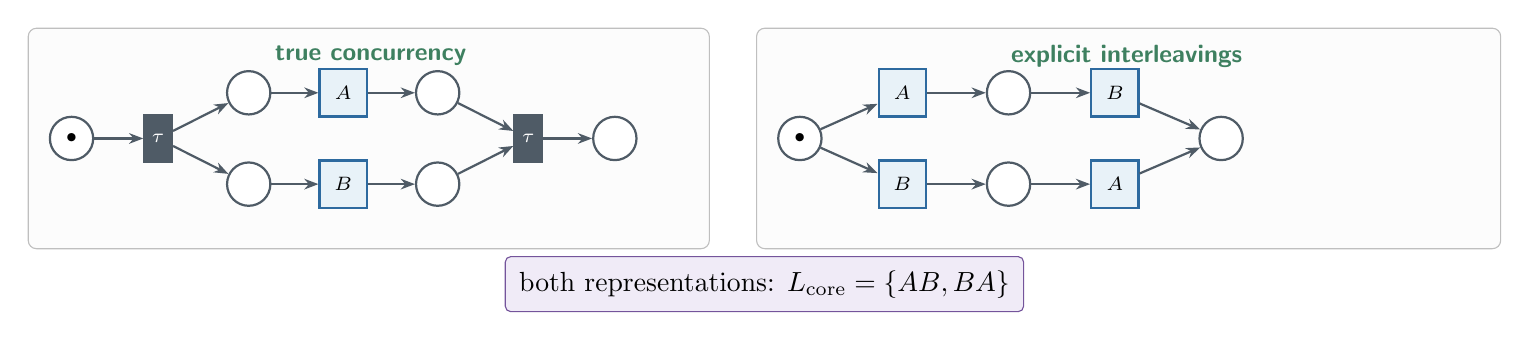
\begin{tikzpicture}
  \draw[draw=black!25, rounded corners=3pt, fill=black!1]
    (-0.45,-1.4) rectangle (8.2,1.4);
  \node[font=\small\sffamily\bfseries, text=laraGreen] at (3.9,1.05)
    {true concurrency};
  \node[marked place] (c0) at (0.1,0) {$\bullet$};
  \node[silent transition] (cs) at (1.2,0) {$\tau$};
  \node[place] (cpa) at (2.35,0.58) {};
  \node[place] (cpb) at (2.35,-0.58) {};
  \node[visible transition] (ca) at (3.55,0.58) {$A$};
  \node[visible transition] (cb) at (3.55,-0.58) {$B$};
  \node[place] (cqa) at (4.75,0.58) {};
  \node[place] (cqb) at (4.75,-0.58) {};
  \node[silent transition] (cj) at (5.9,0) {$\tau$};
  \node[place] (cf) at (7.0,0) {};
  \draw[petri arc] (c0) -- (cs);
  \draw[petri arc] (cs) -- (cpa); \draw[petri arc] (cs) -- (cpb);
  \draw[petri arc] (cpa) -- (ca); \draw[petri arc] (ca) -- (cqa);
  \draw[petri arc] (cpb) -- (cb); \draw[petri arc] (cb) -- (cqb);
  \draw[petri arc] (cqa) -- (cj); \draw[petri arc] (cqb) -- (cj);
  \draw[petri arc] (cj) -- (cf);

  \draw[draw=black!25, rounded corners=3pt, fill=black!1]
    (8.8,-1.4) rectangle (18.25,1.4);
  \node[font=\small\sffamily\bfseries, text=laraGreen] at (13.5,1.05)
    {explicit interleavings};
  \node[marked place] (i0) at (9.35,0) {$\bullet$};
  \node[visible transition] (ia1) at (10.65,0.58) {$A$};
  \node[visible transition] (ib1) at (10.65,-0.58) {$B$};
  \node[place] (ipab) at (12.0,0.58) {};
  \node[place] (ipba) at (12.0,-0.58) {};
  \node[visible transition] (ib2) at (13.35,0.58) {$B$};
  \node[visible transition] (ia2) at (13.35,-0.58) {$A$};
  \node[place] (if) at (14.7,0) {};
  \draw[petri arc] (i0) -- (ia1); \draw[petri arc] (i0) -- (ib1);
  \draw[petri arc] (ia1) -- (ipab); \draw[petri arc] (ib1) -- (ipba);
  \draw[petri arc] (ipab) -- (ib2); \draw[petri arc] (ipba) -- (ia2);
  \draw[petri arc] (ib2) -- (if); \draw[petri arc] (ia2) -- (if);
  \node[output box] at (8.9,-1.85)
    {both representations: $L_{\mathrm{core}}=\{AB,BA\}$};
\end{tikzpicture}%
}
\caption{Two representations of the concurrent-versus-interleaved motif.
Independent enabled transitions produce both orders on the left; an exclusive
choice between two fixed paths produces the same visible language on the
right.}
\label{fig:concurrent-interleaved-pair}
\end{figure}

\paragraph{M-pattern.}
This motif compares a block-structured net with a non-free-choice M-pattern.
The visible behavior is an exclusive choice between $B$ and the parallel
execution of $A$ and $C$. The non-free-choice representation shares input
places in a way that violates free choice. This gives the model examples whose
behavior is simple but whose Petri net structure is not block structured.

\begin{figure}[htbp]
\centering
\resizebox{\textwidth}{!}{%
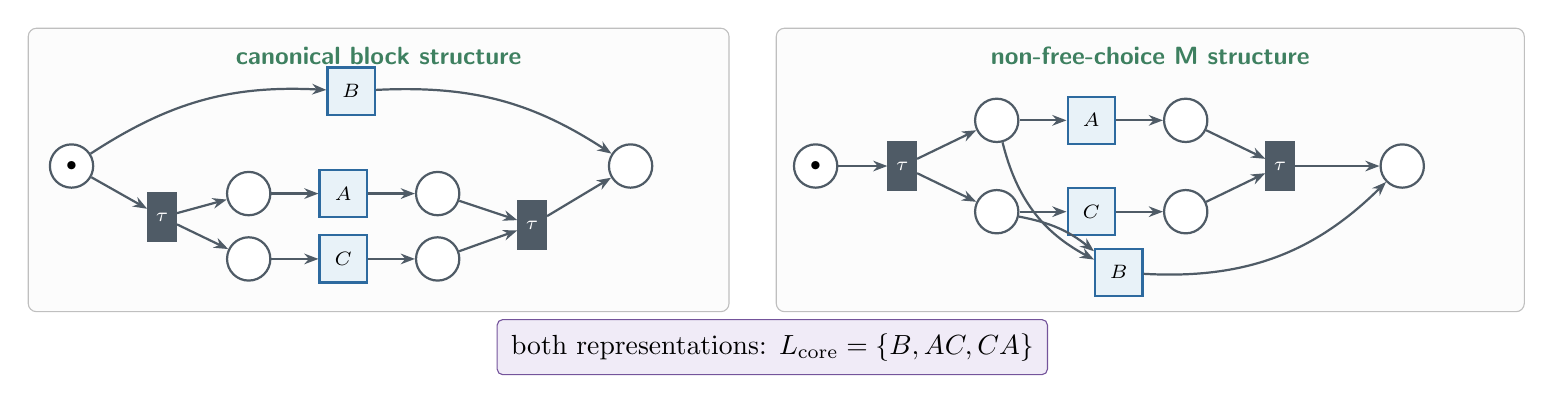
\begin{tikzpicture}
  \draw[draw=black!25, rounded corners=3pt, fill=black!1]
    (-0.45,-1.85) rectangle (8.45,1.75);
  \node[font=\small\sffamily\bfseries, text=laraGreen] at (4.0,1.4)
    {canonical block structure};
  \node[marked place] (m0) at (0.1,0) {$\bullet$};
  \node[visible transition] (mb) at (3.65,0.95) {$B$};
  \node[silent transition] (ms) at (1.25,-0.65) {$\tau$};
  \node[place] (mpa) at (2.35,-0.35) {};
  \node[place] (mpc) at (2.35,-1.18) {};
  \node[visible transition] (ma) at (3.55,-0.35) {$A$};
  \node[visible transition] (mc) at (3.55,-1.18) {$C$};
  \node[place] (mqa) at (4.75,-0.35) {};
  \node[place] (mqc) at (4.75,-1.18) {};
  \node[silent transition] (mj) at (5.95,-0.75) {$\tau$};
  \node[place] (mf) at (7.2,0) {};
  \draw[petri arc] (m0) to[bend left=18] (mb);
  \draw[petri arc] (mb) to[bend left=18] (mf);
  \draw[petri arc] (m0) -- (ms);
  \draw[petri arc] (ms) -- (mpa); \draw[petri arc] (ms) -- (mpc);
  \draw[petri arc] (mpa) -- (ma); \draw[petri arc] (ma) -- (mqa);
  \draw[petri arc] (mpc) -- (mc); \draw[petri arc] (mc) -- (mqc);
  \draw[petri arc] (mqa) -- (mj); \draw[petri arc] (mqc) -- (mj);
  \draw[petri arc] (mj) -- (mf);

  \draw[draw=black!25, rounded corners=3pt, fill=black!1]
    (9.05,-1.85) rectangle (18.55,1.75);
  \node[font=\small\sffamily\bfseries, text=laraGreen] at (13.8,1.4)
    {non-free-choice M structure};
  \node[marked place] (n0) at (9.55,0) {$\bullet$};
  \node[silent transition] (ns) at (10.65,0) {$\tau$};
  \node[place] (np1) at (11.85,0.58) {};
  \node[place] (np2) at (11.85,-0.58) {};
  \node[visible transition] (na) at (13.05,0.58) {$A$};
  \node[visible transition] (nc) at (13.05,-0.58) {$C$};
  \node[place] (nq1) at (14.25,0.58) {};
  \node[place] (nq2) at (14.25,-0.58) {};
  \node[visible transition] (nb) at (13.4,-1.35) {$B$};
  \node[silent transition] (nj) at (15.45,0) {$\tau$};
  \node[place] (nf) at (17.0,0) {};
  \draw[petri arc] (n0) -- (ns);
  \draw[petri arc] (ns) -- (np1); \draw[petri arc] (ns) -- (np2);
  \draw[petri arc] (np1) -- (na); \draw[petri arc] (na) -- (nq1);
  \draw[petri arc] (np2) -- (nc); \draw[petri arc] (nc) -- (nq2);
  \draw[petri arc] (np1) to[bend right=24] (nb);
  \draw[petri arc] (np2) to[bend left=14] (nb);
  \draw[petri arc] (nb) to[bend right=24] (nf);
  \draw[petri arc] (nq1) -- (nj); \draw[petri arc] (nq2) -- (nj);
  \draw[petri arc] (nj) -- (nf);
  \node[output box] at (9.0,-2.3)
    {both representations: $L_{\mathrm{core}}=\{B,AC,CA\}$};
\end{tikzpicture}%
}
\caption{Two representations of the M-pattern motif. In the right net,
$A$ and $B$ share one input place while $B$ and $C$ share another, so the
choice is not free. The complete visible languages still agree.}
\label{fig:m-pattern-pair}
\end{figure}

For each of the three controlled motifs above, the default generator appends
two visible activities in sequence, labeled $D$ and $E$, to both representations.
These labels are fresh relative to that core. If its language is $L_{\mathrm{core}}$,
the full language becomes $\{wDE\mid w\in L_{\mathrm{core}}\}$. For example,
$\{AB,AC\}$ becomes $\{ABDE,ACDE\}$, and $\{B,AC,CA\}$ becomes
$\{BDE,ACDE,CADE\}$. Every clean trace gains two events; language equality
between the paired nets is preserved. The suffix is attached to the core exit,
and its end becomes the new final marking.

\begin{figure}[htbp]
\centering
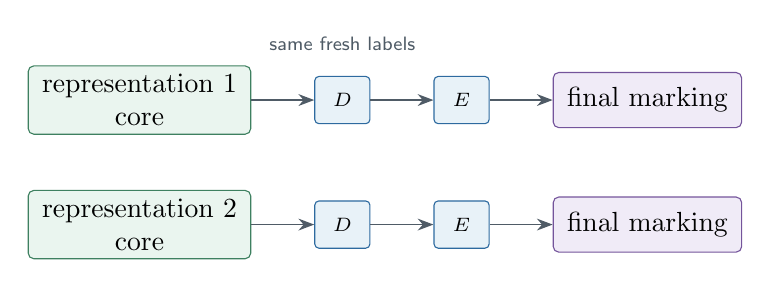
\begin{tikzpicture}[node distance=8mm]
  \node[process box] (core1) {representation 1\\core};
  \node[event, right=of core1] (d1) {$D$};
  \node[event, right=of d1] (e1) {$E$};
  \node[output box, right=of e1] (final1) {final marking};
  \node[process box, below=7mm of core1] (core2) {representation 2\\core};
  \node[event, right=of core2] (d2) {$D$};
  \node[event, right=of d2] (e2) {$E$};
  \node[output box, right=of e2] (final2) {final marking};
  \draw[flow] (core1) -- (d1); \draw[flow] (d1) -- (e1);
  \draw[flow] (e1) -- (final1);
  \draw[flow] (core2) -- (d2); \draw[flow] (d2) -- (e2);
  \draw[flow] (e2) -- (final2);
  \node[tiny label, above=2mm of d1] {same fresh labels};
\end{tikzpicture}
\caption{Shared visible suffix appended to both representations of each
controlled motif. The suffix changes the full traces but not the comparison
between representation structures.}
\label{fig:shared-suffix}
\end{figure}

\subsection{Checking That Representations Match}

After the representations are built, the generator enumerates their visible
complete-trace languages. The default limits for this check are 5,000 search
states, 10,000 traces, and visible length 20; a separate firing bound prevents
unbounded silent exploration. The certificate is \texttt{exact} only when the
enumeration finishes without hitting a bound, and is otherwise
\texttt{bounded}. A family is rejected if the enumerated languages disagree.
A family is also rejected if the reference language is empty, the final
marking is unreachable, or any transition is dead. By default, bounded
certificates are additionally rejected for training; presets intended for
bounded loops can relax that requirement.

\begin{figure}[htbp]
\centering
\resizebox{\textwidth}{!}{%
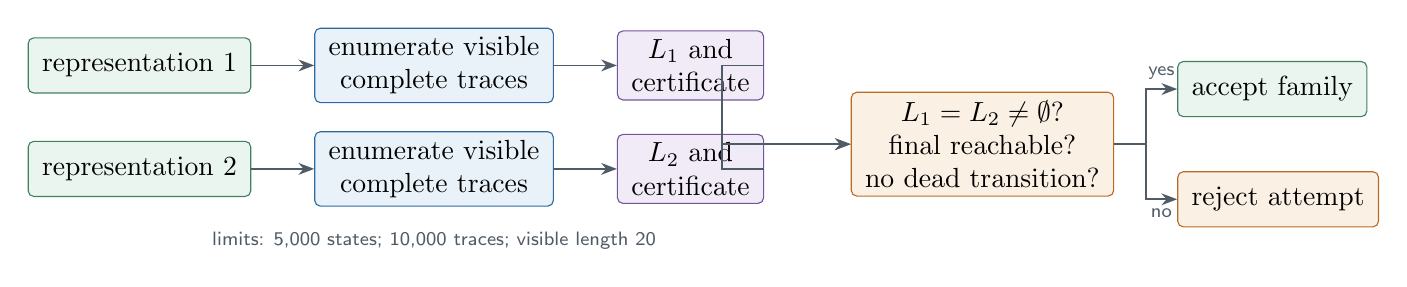
\begin{tikzpicture}[node distance=6mm and 8mm]
  \node[process box] (rep1) {representation 1};
  \node[process box, below=6mm of rep1] (rep2) {representation 2};
  \node[data box, right=of rep1] (enum1) {enumerate visible\\complete traces};
  \node[data box, right=of rep2] (enum2) {enumerate visible\\complete traces};
  \node[output box, right=of enum1] (lang1) {$L_1$ and\\certificate};
  \node[output box, right=of enum2] (lang2) {$L_2$ and\\certificate};
  \node[decision box, right=11mm of lang1, yshift=-10mm] (gate)
    {$L_1=L_2\ne\emptyset$?\\final reachable?\\no dead transition?};
  \node[process box, right=of gate, yshift=7mm] (accept) {accept family};
  \node[decision box, right=of gate, yshift=-7mm] (reject) {reject attempt};
  \draw[flow] (rep1) -- (enum1); \draw[flow] (rep2) -- (enum2);
  \draw[flow] (enum1) -- (lang1); \draw[flow] (enum2) -- (lang2);
  \draw[flow] (lang1) -- ++(4mm,0) |- (gate.west);
  \draw[flow] (lang2) -- ++(4mm,0) |- (gate.west);
  \draw[flow] (gate.east) -- ++(4mm,0) |- node[tiny label, near end, above] {yes} (accept.west);
  \draw[flow] (gate.east) -- ++(4mm,0) |- node[tiny label, near end, below] {no} (reject.west);
  \node[tiny label, below=2mm of enum2]
    {limits: 5,000 states; 10,000 traces; visible length 20};
\end{tikzpicture}%
}
\caption{Family-level representation check. Enumeration records whether each
language result is exact or bounded; default training additionally requires an
exact certificate. A rejected attempt is replaced without changing its planned
motif.}
\label{fig:language-certificate}
\end{figure}

The reference corpus is small enough that all accepted train, validation, and
test rows have an exact visible-language certificate. In other words, the
language comparison completed within the limits for every accepted row.

\subsection{Clean Trace Pool}

For each accepted family, the generator sorts the enumerated visible language
and keeps at most 16 clean traces. If the language has more than 16 traces, a
deterministic sample of 16 indices is selected with the family model RNG and
then restored to language order. These clean traces are not training rows yet.
They are the fitting traces from which observed traces are produced.

The default configuration creates two observed traces per family. The first two
clean traces in the selected pool are used, wrapping around if the pool is
smaller than two. Trace generation is deterministic given the global seed, the
split name, and the family index.

\begin{figure}[htbp]
\centering
\resizebox{\textwidth}{!}{%
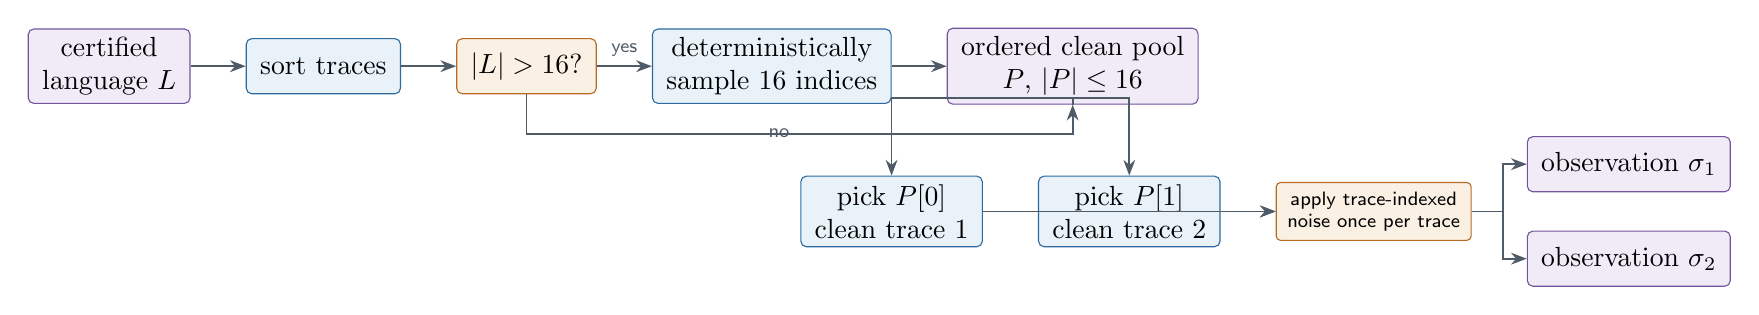
\begin{tikzpicture}[node distance=6mm and 7mm]
  \node[output box] (lang) {certified\\language $L$};
  \node[data box, right=of lang] (sort) {sort traces};
  \node[decision box, right=of sort] (cap) {$|L|>16$?};
  \node[data box, right=of cap] (sample) {deterministically\\sample 16 indices};
  \node[output box, right=of sample] (pool) {ordered clean pool\\$P$, $|P|\leq16$};
  \node[data box, below=9mm of pool, xshift=-23mm] (pick1)
    {pick $P[0]$\\clean trace 1};
  \node[data box, right=of pick1] (pick2)
    {pick $P[1]$\\clean trace 2};
  \node[operation, right=of pick2] (noise)
    {apply trace-indexed\\noise once per trace};
  \node[output box, right=of noise, yshift=6mm] (sig1) {observation $\sigma_1$};
  \node[output box, right=of noise, yshift=-6mm] (sig2) {observation $\sigma_2$};
  \draw[flow] (lang) -- (sort); \draw[flow] (sort) -- (cap);
  \draw[flow] (cap) -- node[tiny label, above] {yes} (sample);
  \draw[flow] (sample) -- (pool);
  \draw[flow] (cap.south) -- ++(0,-5mm) -| node[tiny label, near start, left] {no} (pool.south);
  \draw[flow] (pool) -- ++(0,-4mm) -| (pick1.north);
  \draw[flow] (pool) -- ++(0,-4mm) -| (pick2.north);
  \draw[flow] (pick1.east) -- ++(3mm,0) |- (noise.west);
  \draw[flow] (pick2) -- (noise);
  \draw[flow] (noise.east) -- ++(4mm,0) |- (sig1.west);
  \draw[flow] (noise.east) -- ++(4mm,0) |- (sig2.west);
\end{tikzpicture}%
}
\caption{Construction of the two observations for an accepted family. A small
pool is selected from the certified language, then each selected clean trace is
corrupted once. The resulting $\sigma_1$ and $\sigma_2$ are reused for both
representations.}
\label{fig:clean-pool}
\end{figure}

\subsection{Trace Noise}

Noise is added once at the visible-label level. The same noisy trace is then
paired with every representation in the family. This is important: if a family
has a duplicate-prefix net and a silent-routing net, both nets see the same
observed trace. The exact aligner then decides how that same observation should
be explained on each representation.

With the default noise settings, 20\% of observed traces are kept clean. The
remaining traces receive one, two, or three edits with probabilities 0.5, 0.3,
and 0.2. The edit operations are:
\begin{itemize}
  \item delete one event;
  \item insert an event whose label is already in the family alphabet;
  \item substitute one event label by another label from the family alphabet;
  \item swap two neighboring events;
  \item repeat one event;
  \item remove a prefix;
  \item remove a suffix;
  \item insert the special outside label \texttt{\_\_OOD\_\_}.
\end{itemize}
The first five operations have weight 0.15 each, prefix and suffix truncation
have weight 0.10 each, and outside insertion has weight 0.05. Generated traces
are capped at length 128. An operation is drawn independently at every edit. If
the selected operation is inapplicable to the current trace (for example, a
deletion from an empty trace or a swap in a one-event trace), the implementation
falls back to outside insertion, so every requested edit still produces a
recorded operation. Consequently, the realized outside-insertion frequency can
be higher than its nominal weight on very short traces.

\begin{figure}[htbp]
\centering
\resizebox{\textwidth}{!}{%
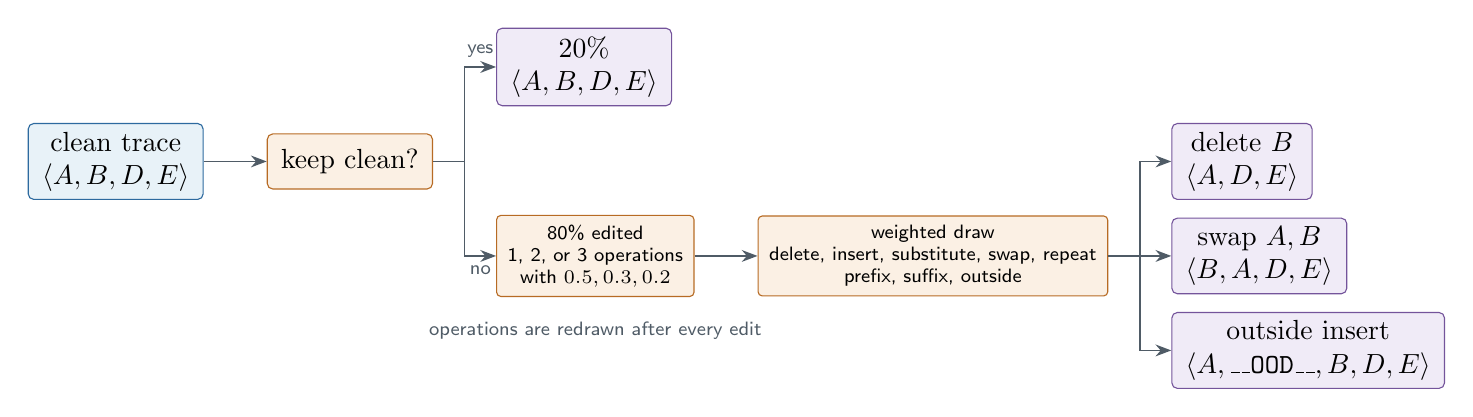
\begin{tikzpicture}[node distance=6mm and 8mm]
  \node[data box] (clean) {clean trace\\$\langle A,B,D,E\rangle$};
  \node[decision box, right=of clean] (keep) {keep clean?};
  \node[output box, right=of keep, yshift=12mm] (unchanged)
    {20\%\\$\langle A,B,D,E\rangle$};
  \node[operation, right=of keep, yshift=-12mm] (edits)
    {80\% edited\\1, 2, or 3 operations\\with $0.5,0.3,0.2$};
  \node[operation, right=of edits] (draw)
    {weighted draw\\delete, insert, substitute, swap, repeat\\prefix, suffix, outside};
  \node[output box, right=of draw, yshift=12mm] (delete)
    {delete $B$\\$\langle A,D,E\rangle$};
  \node[output box, right=of draw] (swap)
    {swap $A,B$\\$\langle B,A,D,E\rangle$};
  \node[output box, right=of draw, yshift=-12mm] (ood)
    {outside insert\\$\langle A,\texttt{\_\_OOD\_\_},B,D,E\rangle$};
  \draw[flow] (clean) -- (keep);
  \draw[flow] (keep.east) -- ++(4mm,0) |- node[tiny label, near end, above] {yes} (unchanged.west);
  \draw[flow] (keep.east) -- ++(4mm,0) |- node[tiny label, near end, below] {no} (edits.west);
  \draw[flow] (edits) -- (draw);
  \draw[flow] (draw.east) -- ++(4mm,0) |- (delete.west);
  \draw[flow] (draw.east) -- (swap.west);
  \draw[flow] (draw.east) -- ++(4mm,0) |- (ood.west);
  \node[tiny label, below=2mm of edits] {operations are redrawn after every edit};
\end{tikzpicture}%
}
\caption{Default trace-corruption mechanism with three illustrative outcomes.
The examples show individual edits; multi-edit observations repeatedly apply
the same weighted operation draw.}
\label{fig:trace-noise}
\end{figure}

\subsection{Exact Labeling}

The initializer expands every accepted family into trace and net pairs and sends
each pair to the PM4Py state-equation A* aligner. The reference generation uses
no per-trace timeout. The aligner is run with transition-aware output enabled,
so the returned alignment identifies the actual Petri net transition used by
each synchronous or model move. Exact results are cached by net signature,
observed label sequence, and cost-model version within each split.

Every exact result is replay-checked by LARA's verifier. Replay checking starts
from the initial marking, fires the model side of the alignment move by move,
checks that the log projection equals the observed trace, and checks that the
final marking is reached. If replay fails, the row is rejected. If PM4Py does
not return an optimal alignment, the whole family is rejected and another
family index is tried. Rows are buffered until every trace and representation pair
in the family passes, so no partial family is written under the default strict
coverage mode.

For families whose representation equivalence was certified exactly, the
initializer also checks cost consistency: the same observed trace must have the
same optimal cost on all equivalent representations. If equivalent
representations disagree in cost, the family is rejected. This prevents the
model from receiving contradictory targets for what is meant to be the same
visible behavior.

\begin{figure}[htbp]
\centering
\resizebox{\textwidth}{!}{%
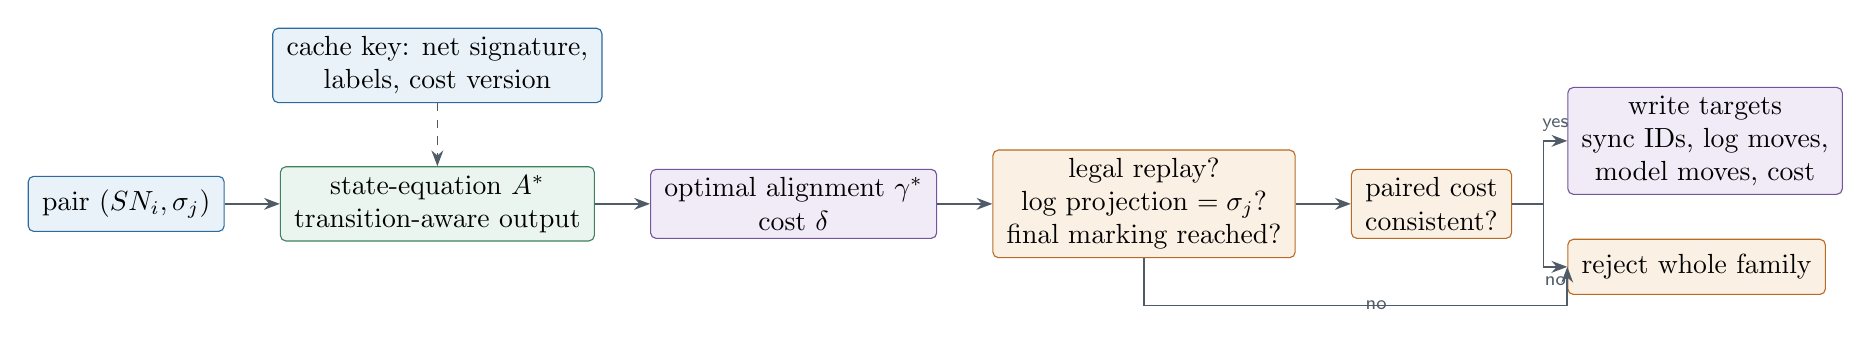
\begin{tikzpicture}[node distance=6mm and 7mm]
  \node[data box] (pair) {pair $(SN_i,\sigma_j)$};
  \node[process box, right=of pair] (astar)
    {state-equation $A^\ast$\\transition-aware output};
  \node[output box, right=of astar] (alignment)
    {optimal alignment $\gamma^\ast$\\cost $\delta$};
  \node[decision box, right=of alignment] (replay)
    {legal replay?\\log projection $=\sigma_j$?\\final marking reached?};
  \node[decision box, right=of replay] (cost)
    {paired cost\\consistent?};
  \node[output box, right=of cost, yshift=8mm] (targets)
    {write targets\\sync IDs, log moves,\\model moves, cost};
  \node[decision box, right=of cost, yshift=-8mm] (reject)
    {reject whole family};
  \node[data box, above=8mm of astar] (cache)
    {cache key: net signature,\\labels, cost version};
  \draw[flow] (pair) -- (astar); \draw[flow] (astar) -- (alignment);
  \draw[flow] (alignment) -- (replay); \draw[flow] (replay) -- (cost);
  \draw[flow] (cost.east) -- ++(4mm,0) |- node[tiny label, near end, above] {yes} (targets.west);
  \draw[flow] (replay.south) -- ++(0,-6mm) -| node[tiny label, near start, right] {no} (reject.west);
  \draw[flow] (cost.east) -- ++(4mm,0) |- node[tiny label, near end, below] {no} (reject.west);
  \draw[flow, dashed] (cache) -- (astar);
\end{tikzpicture}%
}
\caption{Exact-labeling and verification pipeline. Rows are committed only
after every pair in the family passes replay; exactly certified equivalent
representations must also agree on optimal cost.}
\label{fig:exact-labeling}
\end{figure}

\FloatBarrier

\subsection{Masked Transition-Identity Targets}

Most synchronous targets can be used directly. One corner case occurs in the
duplicate-prefix representation. Its $A$ transition is considered identifiable
exactly when the observed labels contain $B$ or $C$, but not both. Noise can
remove both distinguishing labels or introduce both, in which case a particular
optimal $A$ witness is not an identifiable target. The implementation then
masks all synchronous transition-identity targets for that row from the sync
loss. The row is still kept: log-move, model-move, and optimal-cost targets remain active, and the
exact witness remains replay-verified. The metadata records this as
\texttt{transition\_identity\_loss\_masked}.

\begin{figure}[htbp]
\centering
\resizebox{\textwidth}{!}{%
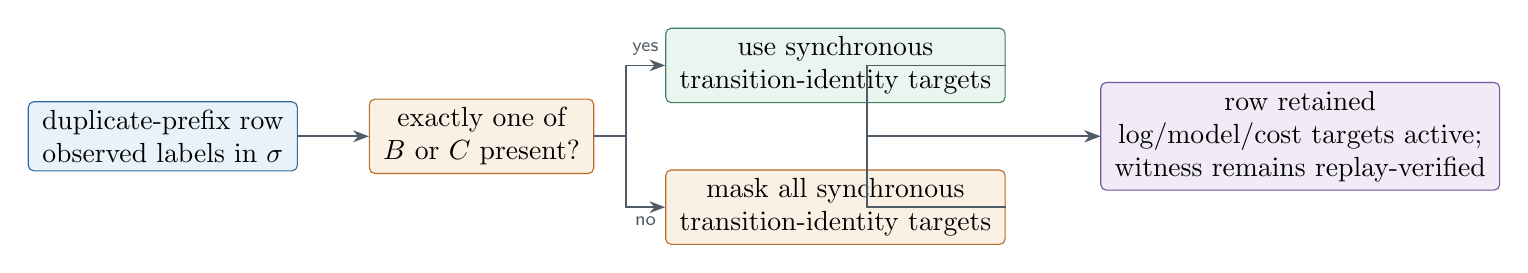
\begin{tikzpicture}[node distance=7mm and 9mm]
  \node[data box] (obs) {duplicate-prefix row\\observed labels in $\sigma$};
  \node[decision box, right=of obs] (xor)
    {exactly one of\\$B$ or $C$ present?};
  \node[process box, right=of xor, yshift=9mm] (active)
    {use synchronous\\transition-identity targets};
  \node[decision box, right=of xor, yshift=-9mm] (masked)
    {mask all synchronous\\transition-identity targets};
  \node[output box, right=12mm of active, yshift=-9mm] (kept)
    {row retained\\log/model/cost targets active;\\witness remains replay-verified};
  \draw[flow] (obs) -- (xor);
  \draw[flow] (xor.east) -- ++(4mm,0) |- node[tiny label, near end, above] {yes} (active.west);
  \draw[flow] (xor.east) -- ++(4mm,0) |- node[tiny label, near end, below] {no} (masked.west);
  \draw[flow] (active) -- ++(4mm,0) |- (kept.west);
  \draw[flow] (masked) -- ++(4mm,0) |- (kept.west);
\end{tikzpicture}%
}
\caption{Masking rule for ambiguous duplicate-prefix observations. Masking
removes only transition-identity supervision, not the row or its other exact
targets.}
\label{fig:identity-mask}
\end{figure}

\FloatBarrier

\subsection{Reference Split Sizes}

The default command
\[
  \texttt{python scripts/init\_data.py --overwrite}
\]
creates the reference corpus in \texttt{data/lara\_synthetic}. It writes the split files \texttt{train.pkl}, \texttt{val.pkl}, and
\texttt{test.pkl}, plus \texttt{metadata.pkl} and \texttt{metadata.json}.

\begin{table}
\centering
\caption{Reference corpus generated with seed 13. Each family expands to four
rows because it has two representations and two observed traces.}
\label{tab:appendix-splits}
\small
\begin{tabular}{@{}lrrr@{}}
\toprule
split & families & rows & families per motif \\
\midrule
train & 512 & 2{,}048 & 128 \\
validation & 128 & 512 & 32 \\
test & 128 & 512 & 32 \\
\bottomrule
\end{tabular}
\end{table}

\begin{figure}[htbp]
\centering
\resizebox{\textwidth}{!}{%
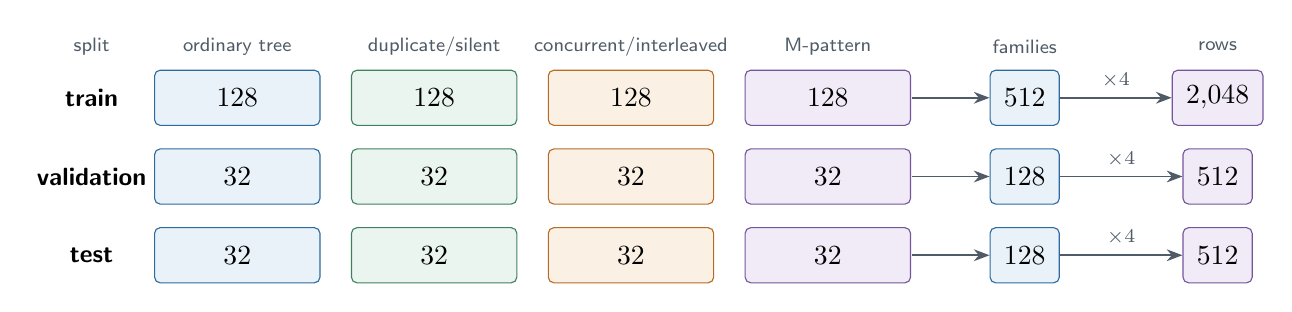
\begin{tikzpicture}
  \node[tiny label] at (0.7,0.65) {split};
  \node[tiny label] at (2.55,0.65) {ordinary tree};
  \node[tiny label] at (5.05,0.65) {duplicate/silent};
  \node[tiny label] at (7.55,0.65) {concurrent/interleaved};
  \node[tiny label] at (10.05,0.65) {M-pattern};
  \node[tiny label] at (12.55,0.65) {families};
  \node[tiny label] at (15.0,0.65) {rows};

  \node[font=\small\sffamily\bfseries] (train) at (0.7,0) {train};
  \node[data box, minimum width=21mm] (to) at (2.55,0) {128};
  \node[process box, minimum width=21mm] (td) at (5.05,0) {128};
  \node[decision box, minimum width=21mm] (tc) at (7.55,0) {128};
  \node[output box, minimum width=21mm] (tm) at (10.05,0) {128};
  \node[draw=none, fit=(to)(tm), inner sep=0pt] (tgroup) {};
  \node[data box] (tf) at (12.55,0) {$512$};
  \node[output box] (tr) at (15.0,0) {$2{,}048$};
  \draw[flow] (tgroup.east) -- (tf.west);
  \draw[flow] (tf) -- node[tiny label, above] {$\times4$} (tr);

  \node[font=\small\sffamily\bfseries] (val) at (0.7,-1.0) {validation};
  \node[data box, minimum width=21mm] (vo) at (2.55,-1.0) {32};
  \node[process box, minimum width=21mm] (vd) at (5.05,-1.0) {32};
  \node[decision box, minimum width=21mm] (vc) at (7.55,-1.0) {32};
  \node[output box, minimum width=21mm] (vm) at (10.05,-1.0) {32};
  \node[draw=none, fit=(vo)(vm), inner sep=0pt] (vgroup) {};
  \node[data box] (vf) at (12.55,-1.0) {$128$};
  \node[output box] (vr) at (15.0,-1.0) {$512$};
  \draw[flow] (vgroup.east) -- (vf.west);
  \draw[flow] (vf) -- node[tiny label, above] {$\times4$} (vr);

  \node[font=\small\sffamily\bfseries] (test) at (0.7,-2.0) {test};
  \node[data box, minimum width=21mm] (eo) at (2.55,-2.0) {32};
  \node[process box, minimum width=21mm] (ed) at (5.05,-2.0) {32};
  \node[decision box, minimum width=21mm] (ec) at (7.55,-2.0) {32};
  \node[output box, minimum width=21mm] (em) at (10.05,-2.0) {32};
  \node[draw=none, fit=(eo)(em), inner sep=0pt] (egroup) {};
  \node[data box] (ef) at (12.55,-2.0) {$128$};
  \node[output box] (er) at (15.0,-2.0) {$512$};
  \draw[flow] (egroup.east) -- (ef.west);
  \draw[flow] (ef) -- node[tiny label, above] {$\times4$} (er);
\end{tikzpicture}%
}
\caption{Balanced family quotas and row expansion in the reference corpus.
Every family remains wholly inside its assigned split, and every accepted family
contributes four rows.}
\label{fig:split-quotas}
\end{figure}

Strict class coverage is used by default. This means the requested split size
must contain complete families, and every active motif must meet its required
minimum. In the reference corpus all four motifs are exactly balanced in every
split. The manifest records one generation detail that does not affect the
accepted corpus: 25 attempted families raised a generation-time
\texttt{ValueError} and were replaced by later accepted families of the same
planned motifs. No exact-alignment, replay, or paired-cost rejection was
recorded for this run.


\FloatBarrier
\section{Neural Scoring and the Complete Training Loss}
\label{app:loss}

\subsection{From Input Tensors to Fixed Move Scores}

With trained parameters $\theta$, the encoder maps $X(SN,\lambda,\sigma)$
to event vectors $v_i$ and transition vectors $u_j$, each of dimension $d=96$.
Place features receive a linear projection and a place-type embedding.
Transition features receive a linear projection, a transition-type embedding,
and the embedding indexed by $z_T$. Two graph blocks combine global
self-attention and typed arc messages. For node $v$, the message term is
\[
 \mu_v=\frac{\sum_{(u,v,r)\in E}W_r h_u}
 {\max(1,|\{(u,v,r)\in E\}|)}.
\]
Each block adds attention and $\mu_v$ through a residual connection and layer
normalization, followed by a residual feed-forward block. A one-layer trace
transformer processes label embeddings plus position embeddings with no causal
mask. Two cross-attention modules let events attend to transitions and
transitions attend to events. Hence both outputs depend on the whole trace,
including future events, and on the net's topology, labels, initial/final
markings, and transition costs.

The heads in \texttt{lara\_align/model.py} compute
\[
\begin{split}
 \mathrm{sync}_\theta(i,t_j\mid SN,\lambda,\sigma)=S_{ij}
 &=\begin{cases}(Wv_i)^\top u_j/\sqrt d,&C_{ij}=1,\\-10^9,&C_{ij}=0,\end{cases}\\
 \mathrm{model}_\theta(t_j\mid SN,\lambda,\sigma)=M_j&=w_M^\top u_j+b_M,\\
 \ell_i&=w_L^\top v_i+b_L.
\end{split}
\]
Dropout is applied during training and disabled at inference. At inference one
forward pass gives $S\in\mathbb{R}^{n\times|T|}$,
$M\in\mathbb{R}^{|T|}$, and $\ell\in\mathbb{R}^n$. The current decoder uses
only $S,M$, reusing them at every visited marking. Its enabledness checks and
bounded searches depend on the current marking; the neural scores do not.
The model-move vector is conditioned on the trace but is not indexed by event
position. The main paper's worked decoding figure lists all move scores for a
complete example, including the unused log scores.

\subsection{Move Imitation}

Use the target conventions of Section~\ref{app:concrete-input}. Let
$I=\{i:y_i\geq0\}$ and $J_i=\{j:C_{ij}=1\}$. In the following equations,
$y_i$ identifies its corresponding transition column, accounting for the
stored zero-based indices. For $i\in I$, define
\[
 p_{ij}=\frac{\exp S_{ij}}{\sum_{k\in J_i}\exp S_{ik}},\qquad j\in J_i.
\]
The implementation uses a finite $-10^9$ sentinel outside $J_i$; its softmax
contribution underflows to zero. With smoothing $\epsilon_s=0.05$,
\[
 \mathcal L_{\mathrm{sync}}=-\frac{1}{|I|}\sum_{i\in I}
 \left[(1-\epsilon_s)\log p_{i,y_i}
 +\frac{\epsilon_s}{|J_i|}\sum_{j\in J_i}\log p_{ij}\right].
\]
Set this term to zero if $I$ is empty. For the concrete row, $I=\{1,2,4\}$;
only the first event offers two compatible transitions. Its smoothed target
masses are $0.025$ on $A_L$ and $0.975$ on $A_R$. Events with a unique
compatible transition contribute zero synchronous cross-entropy.

For a raw logit $z$ and binary target $u$, write
$\operatorname{BCE}(z,u)=\log(1+e^z)-uz$, evaluated numerically in its stable
form. With binary smoothing $\epsilon_b=0.03$, set
$\widetilde u=(1-2\epsilon_b)u+\epsilon_b$. The other move losses are
\[
 \mathcal L_{\mathrm{log}}=\frac1n\sum_{i=1}^n
   \operatorname{BCE}(\ell_i,0.94q_i+0.03),\qquad
 \mathcal L_{\mathrm{model}}=\frac1{|T|}\sum_{j=1}^{|T|}
   \operatorname{BCE}(M_j,0.94b_j+0.03).
\]
An empty output contributes zero. For the concrete row, smoothing gives
\[
 \widetilde q=(0.03,0.03,0.97,0.03),\qquad
 \widetilde b=(0.03,0.97,0.03,0.03,0.03,0.03).
\]
Log loss has the same weight as the other move losses, even though the decoder
does not consume its scores.

\subsection{Auxiliary Cost and Region Terms}

A learned router assigns each transition and event a softmax distribution
over $R=6$ latent regions, denoted $Q^T_{jr}$ and $Q^E_{ir}$. Each region
forms normalized weighted means of its transition and event vectors,
concatenates them, and applies a small feed-forward network to obtain $h_r$.
The denominator of each weighted mean is clamped below at $10^{-6}$.
Two softplus heads give $\widehat l_r\geq0$ and
$\widehat u_r=\widehat l_r+\operatorname{softplus}(w_u^\top h_r+b_u)$.
These are learned endpoints, not admissible bounds. Only the sum of upper
endpoints is supervised against the optimal cost:
\[
 \widehat c=\sum_{r=1}^R\widehat u_r,\qquad
 \mathcal L_{\mathrm{cost}}=H_1(\widehat c-\delta),\qquad
 H_1(e)=\begin{cases}\tfrac12e^2,&|e|<1,\\|e|-\tfrac12,&|e|\geq1.\end{cases}
\]
The implementation also exposes sketch and uncertainty heads; neither has a
direct supervised loss or enters the current decoder.

For each place $p$, let $U_p$ be the set of distinct incident transitions,
regardless of arc direction. Boundary regularization averages over all
unordered transition pairs within each $U_p$:
\[
 \mathcal L_{\mathrm{boundary}}=
 \frac{\displaystyle\sum_{p\in P}\sum_{\{j,k\}\subseteq U_p}
       \left(1-\sum_{r=1}^R Q^T_{jr}Q^T_{kr}\right)}
      {\displaystyle\sum_{p\in P}\binom{|U_p|}{2}}.
\]
A pair sharing several places appears once for each such place; if there are
no pairs the term is zero. It encourages incident transitions to share regions.
Let the mean region load over transitions and events be
$a_r=(\sum_j Q^T_{jr}+\sum_i Q^E_{ir})/(|T|+n)$. Then
\[
 \mathcal L_{\mathrm{balance}}=\frac1R\sum_r(a_r-1/R)^2,\qquad
 \mathcal L_{\mathrm{entropy}}=\tfrac12
 \left[\frac1{|T|}\sum_j H(Q^T_j)+\frac1n\sum_i H(Q^E_i)\right],
\]
where $H(q)=-\sum_r q_r\log q_r$ (logs are clamped at $10^{-8}$ in code).
For an empty trace, balance and entropy use only transitions. The positive
entropy weight encourages concentrated assignments; balance discourages
collapse into a single region.

\subsection{Total Loss and Optimization Settings}

The reference command uses the following complete objective:
\[
\begin{split}
\mathcal L={}&\mathcal L_{\mathrm{sync}}+\mathcal L_{\mathrm{log}}
 +\mathcal L_{\mathrm{model}}+0.03\mathcal L_{\mathrm{cost}}\\
 &+0.01\mathcal L_{\mathrm{boundary}}+0.01\mathcal L_{\mathrm{balance}}
 +0.001\mathcal L_{\mathrm{entropy}}.
\end{split}
\]
Each component is reduced per input pair as above, then averaged over the
16 pairs in an optimizer step (the implementation processes each pair
separately and accumulates gradients). AdamW uses learning rate $5\times10^{-4}$,
weight decay $3\times10^{-3}$, and gradient-norm clipping at 1. Dropout is
$0.30$. Validation loss controls learning-rate reduction by factor $0.5$ after
two plateau epochs (minimum $10^{-5}$) and early stopping with patience six
and minimum improvement $5\times10^{-4}$. The seed is 13; the reference run
executes 50 epochs and selects epoch 49. The settings are defined in
\texttt{scripts/train\_model.py}; the loss reductions and masking are defined in
\texttt{lara\_align/training.py}. Neither replay legality nor exact certification
is a differentiable training term: both are explicit semantic checks outside
the neural objective.

\end{document}
